\documentclass[10pt]{article}
\usepackage[margin=0.65in]{geometry}
\usepackage{amsmath,amssymb,booktabs,graphicx,array,longtable,fancyvrb,listings}
\usepackage[hidelinks]{hyperref}
\setlength{\parindent}{0pt}
\setlength{\parskip}{3pt}
\setlength{\emergencystretch}{2em}
\makeatletter
\renewcommand\section{\@startsection{section}{1}{0pt}{1.2ex plus .5ex minus .2ex}{.6ex plus .2ex}{\normalfont\large\bfseries}}
\makeatother
\newcommand{\code}[1]{\nolinkurl{#1}}
\newcommand{\NoMargin}{0.10717}
\newcommand{\YesMargin}{0.11}
\newcommand{\ConceptTrainCount}{8}
\newcommand{\ConceptTestCount}{9}
\newcommand{\ParaphraseDescription}{GPT-6.1-sol generated one paraphrase for each of 100 fixed test sources (25 per dataset/class, seed 15), using the earlier override-paraphrase toy example as inspiration. No detector scores were used to select variants. Automated review judged intent preserved for 100/100, but agreed with only 83/100 publisher labels under the narrower override definition. The disagreements concern original positive examples whose standalone intent is ambiguous, such as a training-date question. Preserve publisher labels; these data do not establish independently verified semantic ground truth.}
\newcommand{\ParaphrasePlanStatus}{Done}
\newcommand{\ParaphrasePlanDate}{Nov. 20}
\newcommand{\GenerationDisclosure}{GPT-6.1-sol generated the 100 paraphrases and supplied automated intent/concept-pair reviews through the author-provided local API. Review prompts and all generated texts/judgments are retained in the data notebook and CSVs.}
\newcommand{\ThresholdDescription}{Frozen threshold: \texttt{0.37308203458513201}; seed-15 LoRA: \texttt{0.50968770950539799}; zero-shot: \texttt{0.4724093079566955}. LoRA seeds 16/17 use \texttt{0.4998234929255746}, \texttt{0.49177553307711619}, respectively.}
\newcommand{\RandomReferenceDescription}{Cells with AP at/below its random reference or AUROC at/below 0.5: frozen: \code{deepset\_base64}, \code{safeguard\_base64}, \code{safeguard\_zero\_width}; lora: \code{deepset\_base64}, \code{safeguard\_base64}, \code{safeguard\_zero\_width}; zero\_shot: \code{deepset\_base64}, \code{deepset\_homoglyph}, \code{deepset\_zero\_width}, \code{safeguard\_homoglyph}, \code{safeguard\_zero\_width}. Obfuscation/tokenization shift and widespread benign false alarms undermine the trained probes; the generic English NLI readout also struggles on this mixed-language task. These are explanations to investigate, not established causes. Frozen and LoRA FPR reach 1.0 on both base64 sets and almost all zero-width cases; high injection recall there is not useful resistance.}
\newcommand{\DriftDescription}{LoRA mean relative drift ranges from 0.0402 to 0.0505 across datasets/seeds. Point-estimate verdicts follow the stated rule; intervals and seed variation must also be considered. A borderline yes whose interval crosses 0.05 does not establish a stable substantial effect. Positive drift establishes movement relative to the frozen reference, not improved detection.}
\newcommand{\ConceptDescription}{For the frozen mean direction, the held-out gap is 3.168 clean and 1.106 under homoglyphs. LoRA homoglyph gaps range 1.063--1.073; mean-direction changes range 0.0007--0.0022. The concept norm is 5.459 frozen versus 5.396--5.458 after LoRA. Neither a larger concept norm nor a stable direction alone demonstrates robustness.}
\newcommand{\FigureFinding}{LoRA changes deepset homoglyph AUROC from 0.7768 to 0.7738 (-0.0030), below the practical improvement threshold; the confidence intervals show substantial uncertainty.}
\newcommand{\ClaimDescription}{Under publisher labels, this one-epoch LoRA pilot produces no practical AUROC improvement in the 8 evaluated perturbation columns under the +0.11 rule, despite measurable representation drift; this does not prove equivalence or rule out stronger PEFT schedules.}
\newcommand{\ErrorSampleDescription}{The sample contains 10 false positives and 2 false negatives.}
\newcommand{\ErrorFinding}{The sampled false alarms include ordinary German and English requests, while the missed injections include explicit and implicit redirection. This points to investigating language balance and tokenization alongside override semantics, rather than treating a high clean AUROC as semantic validation.}
\newcommand{\BaselineReproduction}{Clean AUROC reproduces the midsemester results to four decimals; maximum probability difference is 0.000884, so thresholds are recalibrated on validation rather than assuming bitwise CPU/GPU agreement.}
\newcommand{\TruncationDescription}{At the shared 128-token encoder budget, changed-text truncation counts are base64 145/315; homoglyph 85/315; paraphrase 4/100; zero\_width 116/315. Truncation is therefore part of the measured stress condition, not an isolated semantic perturbation effect.}
\newcommand{\ComputeDescription}{The measured LoRA training mean is $B=0.175$ min and extraction mean $E=0.399$ min. For three seeds and three epochs, provisionally budget $9B$ each for adapters and prompt/prefix tuning; allow $72B$ for full fine-tuning (eight times the restricted pilot's epoch cost), $9E$ for extraction across the nine added runs, and 4 min for lexical/external checks and visualization. Total: $90B+9E+4=23.4$ T4 minutes. API-generation latency and manual review are additional wall time.}

\begin{document}
\begin{center}
{\large\bfseries Understanding Prompt-Injection Detection using LLM-encoded Representations}\\[3pt]
{\bfseries Project 15: Final Checkpoint}\\
Quang Hung Bui \quad COSC 4371, Fall 2026 \quad November 20, 2026\\
\url{https://github.com/hungqbui/security_anaylytics_project}
\end{center}

\fontsize{9}{10.3}\selectfont
\section{Main comparison}
\textbf{Question.} Where does LoRA fine-tuning remain intolerant to intent-preserving perturbations, and what do learned injection-concept representations reveal about these failures? Clean AUROC near 0.99 motivates testing perturbations rather than expecting a meaningful gain at the clean ceiling.

\textbf{(a) Scope change, what ran and what stayed fixed.} To keep the focus simple and accommodate limited compute resources, narrow the planned comparison to four methods: frozen DeBERTa, LoRA, zero-shot NLI, and a standard full fine-tuning baseline. Defer adapters and prompt/prefix tuning. The goal is to examine LoRA's perturbation intolerance through its learned injection-concept representations, including whether adaptation improves ranking while leaving concept separation or benign decisions fragile. This is a question to test, not an assumption that LoRA necessarily reduces robustness.

Completed comparisons use frozen DeBERTa plus a logistic probe (\code{frozen}) and LoRA plus the same probe-fitting protocol (\code{lora}). An auxiliary \code{zero\_shot} detector uses pretrained NLI weights with class descriptions and no prompt-injection training. It is an external control rather than a controlled encoder-adaptation value. Full fine-tuning remains planned; it will use the same data boundaries, pooling and probe evaluation. Score every method on identical rows within each column: clean, zero-width, homoglyph and base64 copies of both datasets, plus the generated-paraphrase subset. Changed copies retain their original IDs and labels. The main checker comparison uses seed 15; seeds 15, 16 and 17 separately assess adaptation stability. They are repetitions, not additional values of the adaptation variable.

Retain the midsemester 1,640 rows: 1,056 training, 269 validation and 315 test rows (116 deepset; 199 Safe-Guard). Use the pinned data/model revisions and exact split construction in the notebooks: seed 15, publisher test partitions, stratified 20\% validation within publisher training, fixed Safe-Guard 800/200 subsamples, and cross-boundary duplicate-group removal. The main encoder is \code{microsoft/deberta-v3-base}, revision \code{8ccc9b6f36199bec6961081d44eb72fb3f7353f3}. Training data, pretrained initialization, 128-token truncation, inference batch 32, last-layer nonspecial/nonpadding mean pooling, test rows and probe hyperparameters remain fixed. No perturbations enter gradient-based weight fitting; they are used for validation selection and testing. Changes since midsemester: replace the one-epoch budget pilot with 20-epoch validation-selected LoRA and perturbation columns; use higher AUROC as the direction of interest because the present question concerns improvement. Section 6 gives the reduced remaining plan.

LoRA updates query/value projections in the last two encoder layers: rank 4, scaling 8, dropout 0.05, 24,576 adapter parameters, training batch 8, 20 epochs. A temporary weighted-BCE head supplies the adaptation loss and is discarded. Each final/epoch probe uses training-only StandardScaler and balanced logistic regression ($C=1$, $L_2$, lbfgs, 2,000 iterations). Split original validation rows 50/50 by dataset/label (seed 15), assigning related groups to one role. \ValidationRolesDescription\ Retain the epoch with highest mean selection AUROC across clean/zero-width/homoglyph/base64 copies; clean probe log loss breaks ties. The restored state is scored on test only after selection. Appendix C gives the optimizer details and full learning curves. Runs use Colab NVIDIA L4, Python 3.13.16, with packages in \code{requirements.txt}.

\textbf{Perturbations.} Zero-width inserts U+200B between consecutive ASCII letters. Homoglyph substitution replaces lowercase a/e/o/p/c/x by visually similar Cyrillic letters. Both operate deterministically on every test text, including negatives. Base64 encodes the full UTF-8 request and prepends an instruction to decode and execute it. Its label refers to the decoded request; this is a separate encoding stress test because execution/decoding context and truncation can alter the operative task. \ParaphraseDescription

\textbf{(b) Thresholds.} Positive class 1 is the publisher's injection label; higher scores mean more likely injection. Every detector selects its own threshold on a separate clean calibration subset: the lowest observed score with benign FPR at most 5\%. Reuse that threshold on every changed test column. \ThresholdDescription\ The zero-shot control uses \href{https://huggingface.co/MoritzLaurer/DeBERTa-v3-base-mnli-fever-anli}{Laurer et al. DeBERTa-v3-base NLI model}, revision \code{6f5cf0a2b59cabb106aca4c287eed12e357e90eb}. Pair each text with fixed benign/injection hypotheses and softmax the two entailment logits; the injection probability is the score. Use a 128-token combined premise/hypothesis budget, truncating only the premise, batch 8. Only threshold calibration uses validation labels. Its NLI training and English-language focus differ from the main encoder setup, so this control cannot causally partition dataset and encoder effects.

\textbf{(c) Leakage.} LoRA uses the \emph{same training set}. After duplicate removal, baseline train--test exact-text overlaps and train--validation overlaps are both 0 across pooled datasets; normalized-text, similarity-component and truncated-token overlap checks are also 0. LoRA inherits those same input boundaries. Concept reference pairs use training sources only; held-out concept sources are separate test rows. The zero-shot control fits no encoder or classifier on this project's training labels. These checks explain near-perfect-metric warnings; they cannot exclude unobserved source families, pretraining contamination or lexical shortcuts.

\newpage
\textbf{(d) Primary metric and results.} AUROC is the unchanged primary metric. Intervals are the final checker's 1,000-resample, row-bootstrap 95\% intervals; a column has one variant per source row. LoRA and zero-shot cells use their own thresholds, but AUROC itself is threshold independent. Paraphrase subsets have 25 positives/25 negatives per dataset when present; full deepset has 60/116 positives (51.72\%), Safe-Guard 63/199 (31.66\%). The 25 examples per class in each paraphrase column limit interval precision and power.
\begin{center}\resizebox{\linewidth}{!}{\begin{tabular}{lccccc}
\toprule
\multicolumn{6}{l}{\textbf{deepset}}\\
Method & Clean & Zero-width & Homoglyph & Base64 & Paraphrase\\\midrule
Frozen probe & 0.9917 [0.9781, 0.9994] & 0.7673 [0.6650, 0.8535] & 0.7768 [0.6878, 0.8569] & 0.4762 [0.3688, 0.5831] & 0.9856 [0.9566, 1.0000]\\
LoRA (seed 15) & 0.9923 [0.9797, 0.9997] & 0.7652 [0.6687, 0.8441] & 0.7738 [0.6858, 0.8492] & 0.4702 [0.3672, 0.5751] & 0.9904 [0.9678, 1.0000]\\
Zero-shot NLI & 0.6128 [0.5033, 0.7167] & 0.3878 [0.2775, 0.5012] & 0.4667 [0.3524, 0.5771] & 0.4363 [0.3381, 0.5448] & 0.5584 [0.3889, 0.7264]\\
Adapters & -- & -- & -- & -- & --\\
Prompt/prefix & -- & -- & -- & -- & --\\
Full fine-tuning & -- & -- & -- & -- & --\\
\midrule
\multicolumn{6}{l}{\textbf{safeguard}}\\
Method & Clean & Zero-width & Homoglyph & Base64 & Paraphrase\\\midrule
Frozen probe & 0.9956 [0.9892, 1.0000] & 0.4700 [0.3940, 0.5527] & 0.5431 [0.4578, 0.6257] & 0.4972 [0.4088, 0.5789] & 1.0000 [1.0000, 1.0000]\\
LoRA (seed 15) & 0.9954 [0.9876, 1.0000] & 0.4813 [0.4049, 0.5648] & 0.5651 [0.4840, 0.6504] & 0.4873 [0.4071, 0.5740] & 1.0000 [1.0000, 1.0000]\\
Zero-shot NLI & 0.7870 [0.7014, 0.8673] & 0.2498 [0.1861, 0.3171] & 0.4973 [0.4162, 0.5806] & 0.5487 [0.4594, 0.6331] & 0.6352 [0.4623, 0.7884]\\
Adapters & -- & -- & -- & -- & --\\
Prompt/prefix & -- & -- & -- & -- & --\\
Full fine-tuning & -- & -- & -- & -- & --\\
\bottomrule\end{tabular}
}\end{center}
Bold marks the best AUROC per column; underlining marks the next distinct score. Ties share a rank.
\RandomReferenceDescription\ Score direction was checked: logistic probability column 1 corresponds to label 1; NLI entailment logits follow the configured label map and the injection hypothesis is candidate 1. Scores were not inverted using test outcomes. \FrozenParaphraseFinding

\textbf{(e) Decision rule and verdicts.} The midsemester clean rule was an absolute AUROC change of at least 0.02 for yes, at most 0.00981 for no, intermediate changes inconclusive. Clean gains of 0.02 are impossible at the observed ceiling. As proposed at midsemester, retain a perturbation rule derived solely from frozen results and fixed for this 20-epoch comparison: the widest baseline half-interval across the six zero-width/homoglyph/base64 columns is \NoMargin. A higher-AUROC change $\geq\YesMargin$ is yes; a change $\leq\NoMargin$ is no; intermediate changes are undecided. Changes in the wrong direction are no. These are practical decision thresholds, not significance tests. Apply this fixed rule to paraphrases as a subsequent evaluation without retuning it. The checker changes and verdicts are:
\begin{center}\small\begin{tabular}{lll}
\toprule
Column & LoRA change (verdict) & Zero-shot change (verdict)\\
\midrule
deepset\_base64 & -0.0060 (no) & -0.0399 (no)\\
deepset\_clean & +0.0006 (no) & -0.3789 (no)\\
deepset\_homoglyph & -0.0030 (no) & -0.3101 (no)\\
deepset\_paraphrase & +0.0048 (no) & -0.4272 (no)\\
deepset\_zero\_width & -0.0021 (no) & -0.3795 (no)\\
safeguard\_base64 & -0.0099 (no) & +0.0515 (no)\\
safeguard\_clean & -0.0001 (no) & -0.2086 (no)\\
safeguard\_homoglyph & +0.0221 (no) & -0.0458 (no)\\
safeguard\_paraphrase & +0.0000 (no) & -0.3648 (no)\\
safeguard\_zero\_width & +0.0113 (no) & -0.2202 (no)\\
\bottomrule\end{tabular}
\end{center}

\textbf{Stability across seeds.} The table reports AUROC mean, sample SD and range over three runs; the main checker table remains seed 15 rather than pooling repeated predictions as independent test rows. Frozen lbfgs probing is effectively deterministic with these settings, so its zero seed spread is not evidence about variation across datasets. Three LoRA seeds are descriptive and insufficient for strong population-level claims.
The full per-column seed table is in Appendix B.

\newpage
\textbf{Assigned representation-change result.} For matched original test texts $S$, report
\[
 D_m(S)=\frac1{|S|}\sum_{x\in S}\frac{\|h_m(x)-h_0(x)\|_2}{\|h_0(x)\|_2+10^{-12}}.
\]
Frozen self-drift is exactly 0. Before adaptation, set a separate exploratory practical rule: $D\geq0.05$ indicates substantial movement (yes), $D\leq0.01$ indicates small movement (no), otherwise undecided. These thresholds express 5\%/1\% relative representation movement; they are not a robustness criterion or a threshold selected from observed LoRA outcomes. Each seed's interval resamples test rows 1,000 times (seed 15); seed spread is reported separately.
\begin{center}\small\begin{tabular}{lrll}
\toprule
Dataset & Seed & $D$ [95\% interval] & Drift verdict\\
\midrule
deepset & 15 & 0.1835 [0.1674, 0.2001] & yes\\
safeguard & 15 & 0.1793 [0.1684, 0.1901] & yes\\
deepset & 16 & 0.2191 [0.1981, 0.2407] & yes\\
safeguard & 16 & 0.2073 [0.1934, 0.2211] & yes\\
deepset & 17 & 0.2369 [0.2106, 0.2658] & yes\\
safeguard & 17 & 0.2074 [0.1906, 0.2241] & yes\\
\bottomrule\end{tabular}
\end{center}
\DriftDescription

\textbf{Concept directions and expected interpretation.} Define the concept as attempting to override the intended task/instructions. For \ConceptTrainCount{} training-only source/control pairs, estimate
\[
 v_m=\frac1{K}\sum_{j=1}^{K}[h_m(I_j)-h_m(B_j)],\qquad u_m=v_m/\|v_m\|_2.
\]
This mean-difference construction is related to \href{https://aclanthology.org/2024.acl-long.828/}{contrastive activation addition (Rimsky et al., 2024)}; original \href{https://proceedings.mlr.press/v80/kim18d/kim18d.pdf}{TCAV (Kim et al., 2018)} instead learns a classifier normal. Controls quote the same source injection as inert data and explicitly request analysis without execution. Training and test controls use different fixed wrapper templates; 24 candidate sources per boundary are sampled independently, seed 17, limited to at most 80 whitespace words. Before final evaluation, GPT reviews source override intent and benign-control intent; \ConceptTrainCount{} training and \ConceptTestCount{} test pairs pass. This automated screening improves relevance but does not replace independent human annotation.

The primary concept-change diagnostic compares the frozen and adapted concept directions, independently of their magnitudes:
\[
C_m=\frac{v_0^\top v_m}{\|v_0\|_2\|v_m\|_2}=u_0^\top u_m,\qquad \theta_m=\arccos(C_m).
\]
Similarity 1 means the same direction, 0 orthogonal directions, and $-1$ opposite directions. This is equivalent to one minus the previously reported cosine distance. It measures concept rotation, not whether that rotation improves detection. The table's \emph{axis cosine} compares concept vectors across models; its clean/homoglyph \emph{contrast cosines} instead compare held-out pair differences with each model's own concept direction.

On \ConceptTestCount{} held-out pairs, compare the projected gap $M_m=N^{-1}\sum_i u_m^\top[h_m(I_i)-h_m(B_i)]$, both clean and with homoglyph substitution applied to both pair members. Also report mean contrast cosine to control raw scaling. Each $u_m$ is fixed before held-out evaluation. Useful reorganization should retain separation under perturbation and improve detection; rotation alone is not a benefit.

Retain the midsemester projected-separation change as a secondary measure along the fixed frozen concept direction:
\[
\Delta M_m=\frac1N\sum_i u_0^\top\!\left([h_m(I_i)-h_m(B_i)]-[h_0(I_i)-h_0(B_i)]\right).
\]
Positive $\Delta M_m$ means increased injection--benign separation along $u_0$; negative values mean decreased separation. This fixed-axis change differs from subtracting the table's clean gaps, which use different axes $u_m$ and $u_0$. It also differs from direction rotation $1-u_0^\top u_m$ and overall representation drift $D$.

As a secondary diagnostic inspired by \href{https://arxiv.org/html/2310.01405v4#A3.SS1}{Zou et al.'s Representation Engineering (2023)}, stack normalized pair differences as rows, center them and compute $Z_c=U\Sigma V^\top$. The first \emph{right} singular vector $p_m$ is oriented toward positive training contrasts; report $1-p_0^\top p_m$. Centered PCA measures variation among contrasts and can remove their common mean. It is a candidate direction rather than a guaranteed semantic axis; near-tied singular values and sampling noise can destabilize it.
\begin{center}\resizebox{\linewidth}{!}{\begin{tabular}{lrllllll}
\toprule
Method & Seed & $1-u_0^\top u_m$ & $1-p_0^\top p_m$ & Clean gap & Homoglyph gap & Clean cosine & Homoglyph cosine\\
\midrule
frozen & 15 & 0.0000 & 0.0000 & 3.168 & 1.106 & 0.362 & 0.182\\
lora & 15 & 0.0015 & 0.0012 & 3.238 & 1.072 & 0.365 & 0.177\\
lora & 16 & 0.0007 & 0.0006 & 3.172 & 1.073 & 0.360 & 0.177\\
lora & 17 & 0.0022 & 0.0046 & 3.180 & 1.063 & 0.363 & 0.176\\
\bottomrule\end{tabular}
}\end{center}
\ConceptDescription\ Across all three LoRA seeds, both the held-out homoglyph gap and contrast cosine exceed the frozen baseline. This consistency supports improved retention of the measured injection concept under homoglyph perturbation; a small geometric change can still matter for detection. Clean results are mixed, so the improvement is specific to the perturbed comparison. The shared analysis-wrapper format and small held-out pair set limit how broadly this evidence generalizes to other wording variations. More diverse independently reviewed controls and training-pair bootstrap estimates would test that scope. The attached paper suggestion by Dr. Verma, \href{https://arxiv.org/abs/2508.11667}{GPS}, motivates examining embedding sensitivity; it does not make direction stability a semantic guarantee.

\newpage
\section{Figure}
\begin{center}
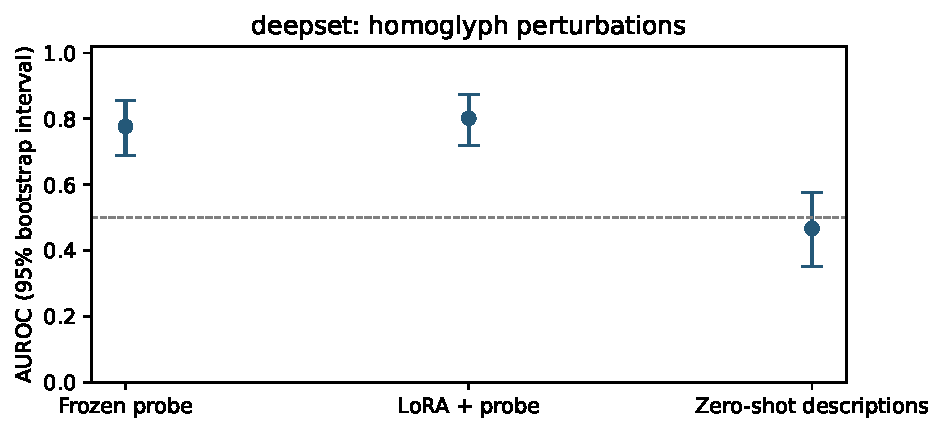
\includegraphics[width=.74\linewidth]{final_comparison.pdf}\\
\small Figure 1. AUROC with checker-matched 95\% intervals for \code{deepset\_homoglyph}: 116 test rows, 60 positive (51.72\%). Values: frozen probe, seed-15 LoRA probe, and zero-shot descriptions.
\end{center}
\FigureFinding

\section{Claim and limitation}
\textbf{(a) Claim.} \ClaimDescription

\textbf{(b) Limitation.} The AUROC gains do not establish reliable detection at the clean-calibrated threshold: Safe-Guard homoglyph FPR rises from 0.5956 to 0.7868, and zero-width FPR remains 1.0000. Thus the positive verdicts concern ranking improvement; threshold transfer and benign false alarms remain unresolved.

\textbf{Interpretation and next check.} Seed-15 homoglyph concept separation improves from 1.106 to 1.151, and contrast cosine from 0.182 to 0.188, with gains in all three seeds. Small geometric changes can matter for classification, although the present results do not isolate their contribution to AUROC. Next, track $D_t$ on fixed validation texts and plot clean/perturbed validation AUROC against epoch and drift, alongside held-out concept separation. Drift with flat or falling perturbed AUROC would indicate movement without detection gains; rising AUROC with retained separation would support useful adaptation. Keep test evaluation separate from epoch selection and report benign false alarms. These trajectories are planned, not existing findings.

\section{Error analysis}
\textbf{(a) Sample.} From \code{frozen / deepset\_homoglyph}, sample 10 false positives and 10 false negatives at random (seed 15), taking all errors of a type when fewer than 10 exist. \ErrorSampleDescription\ Every sampled row appears once in \code{errors.csv}; \code{error\_examples.csv} includes its text and score.

\textbf{(b) Categories.} Categories describe source content rather than proving a causal failure mechanism. Categorize from the original unobfuscated text. ``German benign request'' is a false alarm whose source contains a German cue (wie, wieviele, was, mein, ich, der, kinder, deutschland, gleichberechtigung or verkehrssicherheit); the remaining benign errors in this sample are English requests. ``Explicit override'' contains ignore, previous, prior, system, policy/policies, rules, constraint(s), zuvor or nicht; the remaining missed injections are ``implicit task or role redirection.'' These exclusive operational rules are implemented in the analysis notebook, and examples were inspected for consistency.
\begin{center}\small\begin{tabular}{lrrl}
\toprule
Category & FP & FN & Example row ID\\
\midrule
English benign request & 2 & 0 & deepset:test:10\\
German benign request & 8 & 0 & deepset:test:56\\
explicit override & 0 & 1 & deepset:test:114\\
implicit task or role redirection & 0 & 1 & deepset:test:86\\
\bottomrule\end{tabular}
\end{center}
\ErrorFinding

\newpage
\section{Reproducibility}
\textbf{(a) Files and commands.} Repository: \url{https://github.com/hungqbui/security_anaylytics_project}. Install \code{requirements.txt} outside the notebooks, then run \code{perturbation\_preparation.ipynb}, \code{final\_experiment.ipynb}, \code{zero\_shot\_nli.ipynb} and \code{final\_analysis.ipynb} in order (single-command equivalent in README). Shared \code{data\_preparation.ipynb} supplies downloads, audits and splits via \texttt{\%run}; the pipeline notebooks write \code{split.csv}, \code{scores.csv} and \code{errors.csv}. Generated text/review CSVs fix the reported evaluation set and avoid API regeneration. Regeneration uses the exact notebook prompts, \code{gpt-6.1-sol} at the OpenAI-compatible endpoint configured by \code{API\_URL}, and \code{OPENAI\_API\_KEY}; no credential is committed. Publish the updated executed notebooks and CSVs with the repository before submission.

The baseline is re-extracted and refitted on the L4 rather than mixing old CPU scores with new GPU scores. \BaselineReproduction\ Seeds 15/16/17 affect LoRA initialization, shuffling and dropout; dataset sampling/splitting is seed 15; concept-source sampling is seed 17. Deterministic obfuscation rules have no sampling. No embedding caches or model checkpoint files are necessary to reproduce the pipeline. \TruncationDescription

Download the supplied checker from Canvas and run, from the repository directory, on one line:
\begin{quote}\small\ttfamily
python check\_final\_checkpoint.py --split split.csv --scores scores.csv --errors errors.csv --metric auroc --reference frozen --direction higher
\end{quote}
\textbf{(b) Checker output.} The complete unedited output is included in Appendix A. The numeric AUROC cells and changes in Section 1 match it. Epoch choices and validation-only learning curves appear in Appendix C. Near-perfect-score and weak-random-reference warnings are addressed in Section 1(c)--(d); error-sampling warnings, if any, must be resolved or explained in Section 4.

\section{Plan to finish}
\textbf{(a) Focused remaining work.}
\begin{center}\footnotesize
\begin{tabular}{p{.64\linewidth}ll}\toprule
Task & Status & Finish date\\\midrule
Frozen/LoRA/NLI results, perturbation tests, drift and concepts & Done & Nov. 20\\
Review paraphrase labels and concept controls & Started & Nov. 21\\
Log LoRA $D_t$ and validation AUROC trajectories (three seeds) & Not started & Nov. 21\\
Full fine-tuning baseline on the same clean/perturbed columns & Not started & Nov. 22\\
Compare concept separation, AUROC and benign false alarms & Started & Nov. 22\\
Finalize uncertainty analysis and report & Started & Nov. 22\\\bottomrule
\end{tabular}
\end{center}
The final comparison is frozen versus LoRA versus NLI versus full fine-tuning. Additional PEFT families, external detectors and exploratory visualizations are deferred. All remaining work is scheduled for November 21--22, before November 23. Full fine-tuning and the LoRA drift trajectories have no measured results yet.

\textbf{(b) Measured compute and remaining budget.} Times below exclude downloads, package setup and API generation. Frozen extraction covers the retained originals; LoRA extraction covers originals, deterministic variants and concept pairs. The temporary loss head is excluded from the LoRA parameter count.
\begin{center}\small\begin{tabular}{lrrlll}
\toprule
Method & Seed & Epoch & Optimize min & Select min & Final extract min\\\midrule
frozen & 15 & 0 & 0.000 & 0.000 & 0.132\\
lora & 15 & 13 & 1.692 & 2.659 & 0.216\\
lora & 16 & 17 & 1.703 & 2.671 & 0.216\\
lora & 17 & 18 & 1.713 & 2.672 & 0.217\\
\bottomrule\end{tabular}
\end{center}
\ComputeDescription\ These extrapolations require recalibration after a pilot of each additional method.

\textbf{AI assistance.} OpenAI Codex assisted with experiment implementation, analysis and LaTeX writing under the author's direction. \GenerationDisclosure\ The author must review generated labels, interpretations and the final submission.

\clearpage
\appendix
\section*{Appendix A: complete final checker output}
\lstinputlisting[basicstyle=\ttfamily\scriptsize,breaklines=true,columns=fullflexible,keepspaces=true,showstringspaces=false]{final_checker_output.txt}
\clearpage
\section*{Appendix B: AUROC across training seeds}
Mean, sample standard deviation and range over LoRA seeds 15, 16 and 17. Frozen probing has zero spread at the shown precision.
\begin{center}\small\begin{tabular}{lll}
\toprule
Column & LoRA mean $\pm$ SD & LoRA range\\
\midrule
deepset\_base64 & 0.4614 $\pm$ 0.0656 & 0.3857--0.5003\\
deepset\_clean & 0.9914 $\pm$ 0.0039 & 0.9887--0.9958\\
deepset\_homoglyph & 0.7997 $\pm$ 0.0095 & 0.7893--0.8080\\
deepset\_paraphrase & 0.9952 $\pm$ 0.0032 & 0.9920--0.9984\\
deepset\_zero\_width & 0.7058 $\pm$ 0.0419 & 0.6589--0.7399\\
safeguard\_base64 & 0.4902 $\pm$ 0.0275 & 0.4630--0.5180\\
safeguard\_clean & 0.9956 $\pm$ 0.0005 & 0.9951--0.9961\\
safeguard\_homoglyph & 0.7816 $\pm$ 0.0235 & 0.7581--0.8051\\
safeguard\_paraphrase & 1.0000 $\pm$ 0.0000 & 1.0000--1.0000\\
safeguard\_zero\_width & 0.6126 $\pm$ 0.0163 & 0.5993--0.6308\\
\bottomrule\end{tabular}
\end{center}
\clearpage
\section*{Appendix C: validation-selected training}
\SelectedEpochDescription\ Epoch selection uses only the selection subset; operating thresholds use the separate calibration subset. Test rows never choose the epoch. All seeds complete 20 epochs, even when an earlier epoch is retained.
\begin{center}\small\begin{tabular}{lrlll}
\toprule
Seed & Retained epoch & Best mean AUROC & Epoch-20 mean & Retained clean AUROC\\
\midrule
15 & 13 & 0.7280 & 0.7214 & 0.9943\\
16 & 17 & 0.7009 & 0.6970 & 0.9885\\
17 & 18 & 0.7049 & 0.7025 & 0.9911\\
\bottomrule\end{tabular}
\end{center}
\begin{center}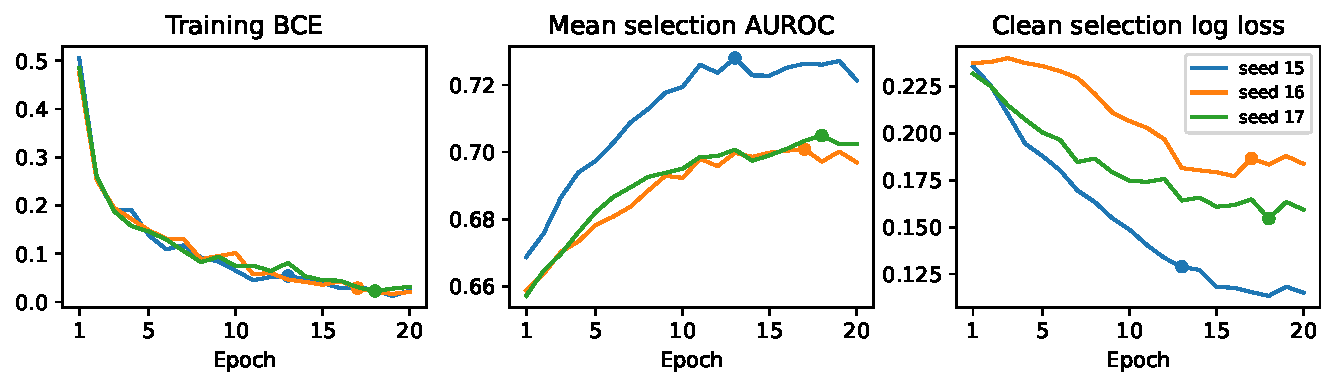
\includegraphics[width=\linewidth]{validation_training_curves.pdf}\end{center}
Optimization uses AdamW: adapter learning rate $10^{-4}$, temporary-head learning rate $10^{-3}$, weight decay 0.01 and gradient clipping 1. The same 1,056 clean rows fit weights in every epoch. Dots mark the retained epoch for each seed. The training loss is the temporary head's weighted BCE; selection AUROC and clean log loss use a freshly fitted training-only logistic probe at each epoch.
\end{document}
